
\section{\label{sec:Taylor}Polinomial Taylor}

Salah satu landasan analisis numerik adalah teorema Taylor yang telah
Anda pelajari dalam Kalkulus. Meskipun demikian, ada baiknya kita
mengulang pembahasan singkatnya di sini.
\begin{thm}
\label{thm:Taylors}\index{Teorema!Taylor}Untuk suatu bilangan bulat
$n\geq0$, misalkan $f(x)$ memiliki $n+1$ turunan pada $(a,b)$,
dan $x_{0}\in(a,b)$. Maka, untuk setiap $x\in(a,b)$, terdapat suatu
$\xi$ yang bergantung pada $x$ dan terletak di antara $x$ dan $x_{0}$
sedemikian sehingga
\[
f(x)=f(x_{0})+\sum_{j=1}^{n}\left(\frac{f^{(j)}(x_{0})}{j!}(x-x_{0})^{j}\right)+\frac{f^{(n+1)}(\xi)}{(n+1)!}(x-x_{0})^{n+1}.
\]
\end{thm}

\begin{proof}
\noindent Untuk kasus $x=x_{0}$, klaim tersebut jelas. $\xi=x=x_{0}$
dapat digunakan. Sekarang misalkan $x\neq x_{0}$, dan misalkan $I$
adalah interval terbuka di antara $x$ dan $x_{0}$, serta $\overline{I}$
adalah interval tertutup di antara $x$ dan $x_{0}$. Karena $I\subset\overline{I}\subset(a,b)$
dan $f$ memiliki $n+1$ turunan pada $(a,b)$, kita memperoleh bahwa
$f,f',f'',\ldots,f^{(n)}$ semuanya kontinu pada $\overline{I}$ dan
bahwa $f^{(n+1)}$ terdefinisi pada $I$. Sekarang kita definisikan
\[
F(z)=f(x)-f(z)-\sum_{j=1}^{n}\frac{f^{(j)}(z)}{j!}(x-z)^{j}
\]
dan kita akan membuktikan teorema dengan menunjukkan bahwa $F(x_{0})=\frac{(x-x_{0})^{n+1}}{(n+1)!}f^{(n+1)}(\xi)$
untuk suatu $\xi\in I$. Perhatikan bahwa $F'(z)$, yang merupakan
jumlah teleskopik, diberikan oleh
\begin{eqnarray*}
F'(z) & = & -f'(z)-\sum_{j=1}^{n}\left[\frac{f^{(j+1)}(z)}{j!}(x-z)^{j}-\frac{f^{(j)}(z)}{(j-1)!}(x-z)^{j-1}\right]\\
 & = & -f'(z)-\left[\frac{f^{(n+1)}(z)}{n!}(x-z)^{n}-f'(z)\right]\\
 & = & -\frac{f^{(n+1)}(z)}{n!}(x-z)^{n}.
\end{eqnarray*}
Sekarang definisikan $g(z)=F(z)-\left(\frac{x-z}{x-x_{0}}\right)^{n+1}F(x_{0})$.
Mudah diperiksa bahwa $g$ memenuhi hipotesis teorema Rolle. Memang,
$g(x_{0})=g(x)=0$ dan syarat kekontinuan serta keterdiferensialan
terpenuhi. Menurut teorema Rolle, terdapat $\xi\in I$ sedemikian
sehingga $g'(\xi)=0=F'(\xi)+(n+1)\frac{(x-\xi)^{n}}{(x-x_{0})^{n-1}}F(x_{0})$.
Dengan demikian, 
\begin{eqnarray*}
F(x_{0}) & = & -F'(\xi)\frac{(x-x_{0})^{n+1}}{(n+1)(x-\xi)^{n}}\\
 & = & \frac{f^{(n+1)}(\xi)}{n!(n+1)}(x-x_{0})^{n+1}\\
 & = & \frac{f^{(n+1)}(\xi)}{(n+1)!}(x-x_{0})^{n+1}.
\end{eqnarray*}
Dengan demikian, pembuktian selesai. 
\end{proof}
Kita akan menggunakan notasi 
\[
T_{n}(x)=f(x_{0})+\sum_{j=1}^{n}\left(\frac{f^{(j)}(x_{0})}{j!}(x-x_{0})^{j}\right)
\]
dan menyebutnya polinomial Taylor berorde $n$ \index{polinomial!Taylor}
\index{Taylor!polinomial} dari $f$ yang dikembangkan di sekitar
$x_{0}$. Kita juga akan menggunakan notasi 
\[
R_{n}(x)=\frac{f^{(n+1)}(\xi)}{(n+1)!}(x-x_{0})^{n+1}
\]
dan menyebutnya suku sisa \index{Taylor!suku sisa} untuk polinomial
Taylor berorde $n$ dari $f$ yang dikembangkan di sekitar $x_{0}$. 

\noindent\begin{digression}{$\xi$}  

\noindent$\xi$ adalah huruf keempat belas (huruf kecil) dalam alfabet
Yunani dan diucapkan \texttt{ksi}. Huruf ini lazim, meskipun tentu
tidak wajib, digunakan untuk besaran yang tidak diketahui dalam teorema
Taylor. Bentuk huruf besar dari $\xi$ adalah $\Xi$, suatu simbol
yang jarang dijumpai dalam matematika. \end{digression}

Demi keringkasan, kita sering menyebut $T_{n}(x)$ sebagai polinomial
Taylor berorde $n$ dan $R_{n}(x)$ sebagai suku sisa ketika fungsi
dan pusat pengembangan $x_{0}$ tidak dinyatakan atau sudah jelas
dari konteks.

Dalam kalkulus, Anda mungkin berfokus pada polinomial Taylor atau
deret Taylor dan tidak terlalu memperhatikan suku sisa. Dalam analisis
numerik, keadaannya justru berkebalikan. Galat algoritmik sering kali
dapat ditentukan dengan mencermati suku sisa, sehingga suku ini menjadi
lebih penting daripada polinomial Taylor itu sendiri. Meskipun demikian,
polinomial Taylor akan digunakan untuk menurunkan metode tertentu
sehingga tidak akan sepenuhnya diabaikan.

Hal terpenting yang perlu dipahami mengenai suku sisa adalah bahwa
suku tersebut menyatakan secara tepat seberapa baik $T_{n}(x)$ menghampiri
$f(x)$. Dari teorema Taylor, $f(x)=T_{n}(x)+R_{n}(x)$, sehingga
galat absolut ketika menggunakan $T_{n}(x)$ untuk menghampiri $f(x)$
diberikan oleh $|T_{n}(x)-f(x)|=|R_{n}(x)|$. Namun, $|R_{n}(x)|=\left|\frac{f^{(n+1)}(\xi)}{(n+1)!}(x-x_{0})^{n+1}\right|$
untuk suatu $\xi$ di antara $x$ dan $x_{0}$. Oleh karena itu, 
\begin{eqnarray*}
|T_{n}(x)-f(x)|=|R_{n}(x)| & \leq & \max_{\xi}\left|\frac{f^{(n+1)}(\xi)}{(n+1)!}(x-x_{0})^{n+1}\right|\\
 & = & \frac{|x-x_{0}|^{n+1}}{(n+1)!}\max_{\xi}\left|f^{(n+1)}(\xi)\right|.
\end{eqnarray*}
Dari pengamatan ini kita memperoleh beberapa hal:
\begin{enumerate}
\item Suku sisa persis merupakan galat yang timbul ketika menggunakan $T_{n}(x)$
untuk menghampiri $f(x)$. Karena itu, suku tersebut kadang-kadang
disebut suku galat\index{Taylor!suku galat}.
\item \label{enu:taylorObservation2}Galat absolut ketika menggunakan $T_{n}(x)$
untuk menghampiri $f(x)$ bergantung pada tiga faktor:

\begin{enumerate}
\item $|x-x_{0}|^{n+1}$
\item $\frac{1}{(n+1)!}$
\item $|f^{(n+1)}(\xi)|$
\end{enumerate}
\item Kita dapat menemukan batas atas bagi $|T_{n}(x)-f(x)|$ dengan menemukan
batas atas bagi $\left|f^{(n+1)}(\xi)\right|$. 
\end{enumerate}
\begin{figure}[h]
\caption{\label{fig:taylor1}Untuk $n$ yang kecil, $T_{n}(x)$ hanya merupakan
hampiran yang baik untuk $x$ yang kecil.}

\begin{centering}
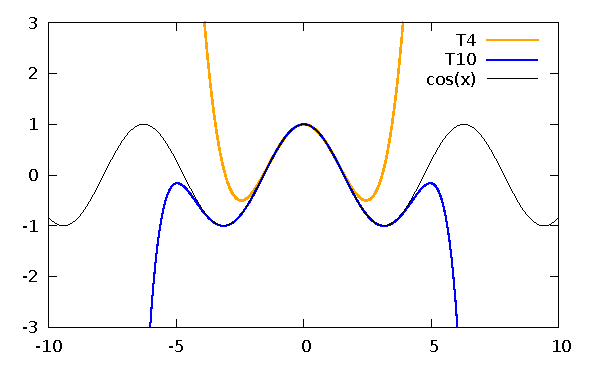
\includegraphics{figures/preliminaries-taylor1}
\par\end{centering}
\end{figure}
 Karena $|R_{n}(x)|$ mengukur secara tepat galat absolut $|T_{n}(x)-f(x)|$,
kita tertarik pada kondisi yang membuat $|R_{n}(x)|$ bernilai kecil.
Menurut pengamatan \ref{enu:taylorObservation2}, ada tiga besaran
yang perlu diperhatikan. Pertama, $|x-x_{0}|^{n+1}$, atau $|x-x_{0}|$,
yaitu jarak antara $x$ dan $x_{0}$. $T_{n}(x)$ pada umumnya memberikan
hampiran yang lebih baik ketika $x$ lebih dekat ke $x_{0}$. Kedua,
$\frac{1}{(n+1)!}$. Hal ini menyiratkan bahwa semakin banyak suku
yang digunakan dalam polinomial Taylor (semakin besar $n$), semakin
baik hampirannya. Terakhir, $|f^{(n+1)}(\xi)|$, yaitu nilai mutlak
turunan berorde $(n+1)$ dari $f$. Semakin terkendali turunan ini,
semakin baik $T_{n}(x)$ menghampiri $f(x)$. Namun, perlu diingat
bahwa semua ini hanyalah pedoman praktis untuk membuat $|R_{n}(x)|$
bernilai kecil. Terdapat pengecualian terhadap pedoman-pedoman tersebut.

Untuk melihat bagaimana ketiga faktor ini bekerja, perhatikan $f(x)=\ln(x)$
yang dikembangkan di sekitar $x_{0}=e^{2}$. Menurut teorema Taylor,
\begin{eqnarray*}
T_{2}(x)=2+\frac{x-e^{2}}{e^{2}}-\frac{(x-e^{2})^{2}}{2e^{4}} & \mbox{ dan } & R_{2}(x)=\frac{1}{3\xi^{3}}(x-e^{2})^{3};\\
T_{11}(x)=2+\sum_{j=1}^{11}\left(\frac{(-1)^{j-1}(x-e^{2})^{j}}{je^{2j}}\right) & \mbox{ dan } & R_{11}(x)=\frac{-1}{12\xi^{12}}(x-e^{2})^{12}.
\end{eqnarray*}
Setelah meyakinkan diri bahwa rumus-rumus ini benar, misalkan kita
ingin menghampiri $\ln(x)$ dengan galat absolut tidak lebih dari
$0.1$. Karena $|\xi^{-3}|$ dan $|\xi^{-12}|$ merupakan fungsi menurun
terhadap $\xi$, keduanya mencapai nilai maksimum pada interval tertutup
di titik ujung kiri interval tersebut. Oleh karena itu, untuk $x\geq e^{2}$,
kita memperoleh $|R_{2}(x)|\leq\max_{\xi\in[e^{2},x]}\left|\frac{1}{3\xi^{3}}(x-e^{2})^{3}\right|=\frac{1}{3e^{6}}(x-e^{2})^{3}$.
Namun, untuk $0<x<e^{2}$, kita memperoleh $|R_{2}(x)|\leq\max_{\xi\in[x,e^{2}]}\left|\frac{1}{3\xi^{3}}(x-e^{2})^{3}\right|=\frac{1}{3x^{3}}(e^{2}-x)^{3}$.
Untuk menentukan nilai peubah yang membuat suku-suku sisa ini lebih
kecil dari $0.1$, kita perlu menyelesaikan persamaan $\frac{1}{3e^{6}}(x-e^{2})^{3}=0.1$
dan $\frac{1}{3x^{3}}(e^{2}-x)^{3}=0.1$. Nilai yang kita cari adalah
$x=\left(1+\sqrt[3]{\frac{3}{10}}\right)e^{2}\approx12.33$ dan $x=\frac{\sqrt[3]{8100}+10\sqrt[3]{90}-30}{13\sqrt[3]{90}}e^{2}\approx4.427$.
Jadi, teorema Taylor menjamin bahwa $T_{2}(x)$ akan menghampiri $\ln(x)$
dengan galat paling besar $0.1$ di seluruh interval $[4.427,12.33]$.
Karena $e^{2}\approx7.389$, $T_{2}(x)$ menghampiri $\ln(x)$ dengan
galat paling besar $0.1$ dari sekitar 3 satuan di bawah $e^{2}$
hingga sekitar 5 satuan di atas $e^{2}$. Dengan kata lain, selama
$x$ cukup dekat dengan $x_{0}=e^{2}$, hampiran tersebut baik. Perhitungan
serupa untuk $R_{11}(x)$ menunjukkan bahwa $T_{11}(x)$ dijamin menghampiri
$\ln(x)$ dengan galat paling besar $0.1$ pada interval $[3.667,14.89]$.
Dengan kata lain, untuk nilai $n$ yang lebih besar, $x$ tidak perlu
sedekat itu dengan $x_{0}$ untuk mencapai akurasi yang sama.

Namun ingatlah, nilai-nilai ini hanyalah batas teoretis bagi galat.
Galat sebenarnya sering kali jauh lebih kecil daripada batas tersebut.
Sebagai contoh, analisis kita memberikan batas atas $|R_{2}(3)|\leq\frac{1}{3\cdot3^{3}}(e^{2}-3)^{3}\approx1.05$
sedangkan galat sebenarnya, $|T_{2}(3)-\ln(3)|=\left|2+\frac{3-e^{2}}{e^{2}}-\frac{(3-e^{2})^{2}}{2e^{4}}-\ln(3)\right|\approx.131$.
Batas tersebut kira-kira 8 kali galat sebenarnya. Jika kita menelaah
hal ini sedikit lebih jauh, grafik $T_{2}(x)$ dan $T_{11}(x)$ dibandingkan
dengan $\ln(x)$ 
\begin{figure}
\caption{\label{fig:taylor3}Galat sebenarnya $|T_{n}(x)-f(x)|$ sering kali
jauh lebih kecil daripada batas teoretis.}

\begin{centering}
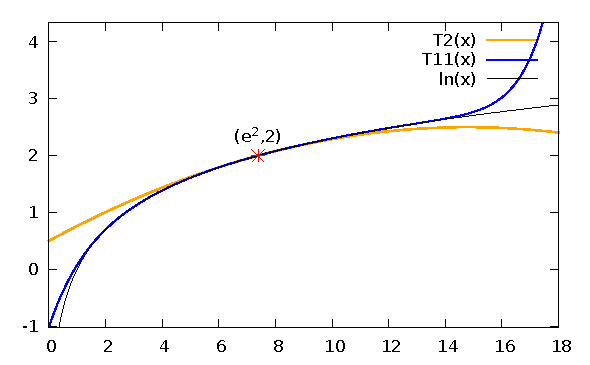
\includegraphics{figures/preliminaries-taylor3}
\par\end{centering}
\end{figure}
 (serta sedikit perhitungan yang akan kita bahas nanti) \label{equationToSolve}
menunjukkan bahwa $T_{2}(x)$ sebenarnya menghampiri $\ln(x)$ dengan
galat paling besar $0.1$ pada interval $[3.296,13.13]$ dan $T_{11}(x)$
sebenarnya menghampiri $\ln(x)$ dengan galat paling besar $0.1$
pada interval $[0.9030,15.33]$. Interval-interval ini sedikit lebih
lebar daripada interval yang dijamin secara teoretis. Lihat Gambar
\ref{fig:taylor3}. Gambar ini juga menunjukkan hal lain. $T_{2}(18)$
jauh lebih baik dalam menghampiri $\ln(18)$ daripada $T_{11}(18)$.
Tidak selalu benar bahwa lebih banyak suku menghasilkan hampiran yang
lebih baik.

Selanjutnya kita membahas polinomial Taylor yang barangkali paling
sering dianalisis---yakni polinomial untuk fungsi sinus dan kosinus.
Keduanya menyajikan contoh dengan visualisasi yang indah dan analisis
yang sederhana.Polinomial Taylor berorde $n$ untuk $f(x)=\cos(x)$
yang dikembangkan di sekitar 0 adalah
\begin{eqnarray*}
T_{n}(x) & = & \cos(0)+\sum_{j=1}^{n}\left(\frac{\left.\frac{d^{j}}{dx^{j}}(\cos(x))\right|_{x=0}}{j!}(x-0)^{j}\right)\\
 & = & \cos(0)-\sin(0)\cdot x-\frac{\cos(0)}{2}x^{2}+\frac{\sin(0)}{6}x^{3}+\frac{\cos(0)}{24}x^{4}-\cdots\\
 & = & 1-\frac{1}{2}x^{2}+\frac{1}{24}x^{4}-\cdots
\end{eqnarray*}
dan suku sisanya adalah 
\begin{eqnarray*}
R_{n}(x) & = & \frac{\left.\frac{d^{n+1}}{dx^{n+1}}(\cos(x))\right|_{x=\xi}}{(n+1)!}(x-0)^{n+1}\\
 & = & \frac{x^{n+1}}{(n+1)!}\begin{cases}
-\sin(\xi) & \mbox{ ketika }n\mbox{ mod }4\equiv0\\
-\cos(\xi) & \mbox{ ketika }n\mbox{ mod }4\equiv1\\
\sin(\xi) & \mbox{ ketika }n\mbox{ mod }4\equiv2\\
\cos(\xi) & \mbox{ ketika }n\mbox{ mod }4\equiv3
\end{cases}.
\end{eqnarray*}
Karena fungsi sinus dan kosinus dibatasi antara $-1$ dan $1$, kita
mengetahui bahwa $-\frac{|x|^{n+1}}{(n+1)!}\leq\frac{x^{n+1}}{(n+1)!}\sin\xi\leq\frac{|x|^{n+1}}{(n+1)!}$
dan demikian pula untuk $-\sin\xi$, $\cos\xi$, serta $-\cos\xi$.
Oleh karena itu, apa pun bentuk suku sisanya,
\[
-\frac{|x|^{n+1}}{(n+1)!}\leq R_{n}(x)\leq\frac{|x|^{n+1}}{(n+1)!}.
\]
Ada dua keadaan yang membuat suku sisa ini bernilai kecil. Pertama,
jika $x$ dekat dengan $0$, maka $|x|$ bernilai kecil sehingga $R_{n}(x)$
bernilai kecil. Kedua, jika $n$ bernilai besar, maka $\frac{1}{(n+1)!}$
bernilai kecil sehingga $R_{n}(x)$ bernilai kecil. Dengan kata lain,
untuk nilai $n$ yang kecil, suku sisanya bernilai kecil ketika nilai
$x$ kecil. $T_{n}(x)$ merupakan hampiran yang baik bagi $\cos(x)$
untuk kombinasi $x$ dan $n$. Sebaliknya, untuk nilai $n$ yang besar,
suku sisanya bernilai kecil bahkan ketika nilai $x$ besar. Sebagai
contoh, $|R_{61}(x)|\leq\frac{|x|^{62}}{62!}$, sehingga $|R_{61}(x)|$
tetap kurang dari 1 untuk semua $x$ yang nilai mutlaknya kurang dari
$\sqrt[62]{62!}\approx23.933$. Gambar \ref{fig:taylor1} dan \ref{fig:taylor2}
mengilustrasikan hal ini. 
\begin{figure}[h]
\caption{\label{fig:taylor2}Untuk $n$ yang besar, $T_{n}(x)$ merupakan hampiran
yang baik bahkan untuk $x$ yang besar.}

\begin{centering}
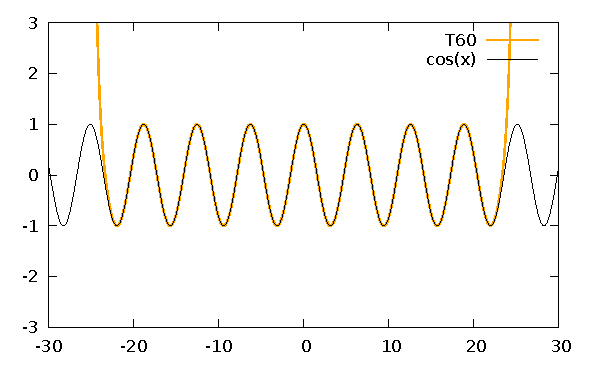
\includegraphics{figures/preliminaries-taylor2}
\par\end{centering}
\end{figure}


\subsection{Konsep Utama}
\begin{description}
\item [{Teorema~Rolle:}] \index{Teorema!Rolle}Misalkan $f(x)$ kontinu
pada $[a,b]$ dan terdiferensialkan pada $(a,b)$. Jika $f(a)=f(b)$,
maka terdapat $\xi\in(a,b)$ sedemikian sehingga $f'(\xi)=0$.
\item [{Teorema~Taylor:}] \index{Teorema!Taylor} Misalkan $f(x)$ memiliki
$n+1$ turunan pada $(a,b)$, dan $x_{0}\in(a,b)$. Maka, untuk setiap
$x\in(a,b)$, terdapat $\xi$, yang bergantung pada $x$, dan terletak
di antara $x$ dan $x_{0}$ tanpa sama dengan keduanya, sedemikian
sehingga
\[
f(x)=f(x_{0})+\sum_{j=1}^{n}\left(\frac{f^{(j)}(x_{0})}{j!}(x-x_{0})^{j}\right)+\frac{f^{(n+1)}(\xi)}{(n+1)!}(x-x_{0})^{n+1}.
\]
\item [{$n$~polinomial~Taylor:}] \index{polinomial!Taylor}\index{Taylor!polinomial}
$T_{n}(x)=f(x_{0})+\sum_{j=1}^{n}\left(\frac{f^{(j)}(x_{0})}{j!}(x-x_{0})^{j}\right)$.
\item [{Polinomial~Maclaurin:}] \index{polinomial!Maclaurin}Polinomial
Taylor yang dikembangkan di sekitar $x_{0}=0$ juga disebut \index{polinomial Maclaurin}polinomial
Maclaurin.
\item [{Suku~sisa:}] $R_{n}(x)=\frac{f^{(n+1)}(\xi)}{(n+1)!}(x-x_{0})^{n+1}$
tepat sama dengan $-\left(T_{n}(x)-f(x)\right)$.
\item [{Suku~galat:}] Nama lain untuk suku sisa.
\end{description}
\begin{digression}{Teorema asli Brook Taylor} 

\noindent Teorema asli \index{Teorema!Taylor} karya Brook Taylor
\index{Taylor!Brook} diterbitkan dalam karya besarnya \textit{Methodus
Incrementorum Directa \& Inversa} pada tahun 1715. Di dalam \textit{Methodus},
teorema ini muncul sebagai korolari kedua dari Proposisi VII Teorema
III dan nyaris tidak menyerupai pernyataan modern mana pun dari teorema
tersebut. 

\begin{center}
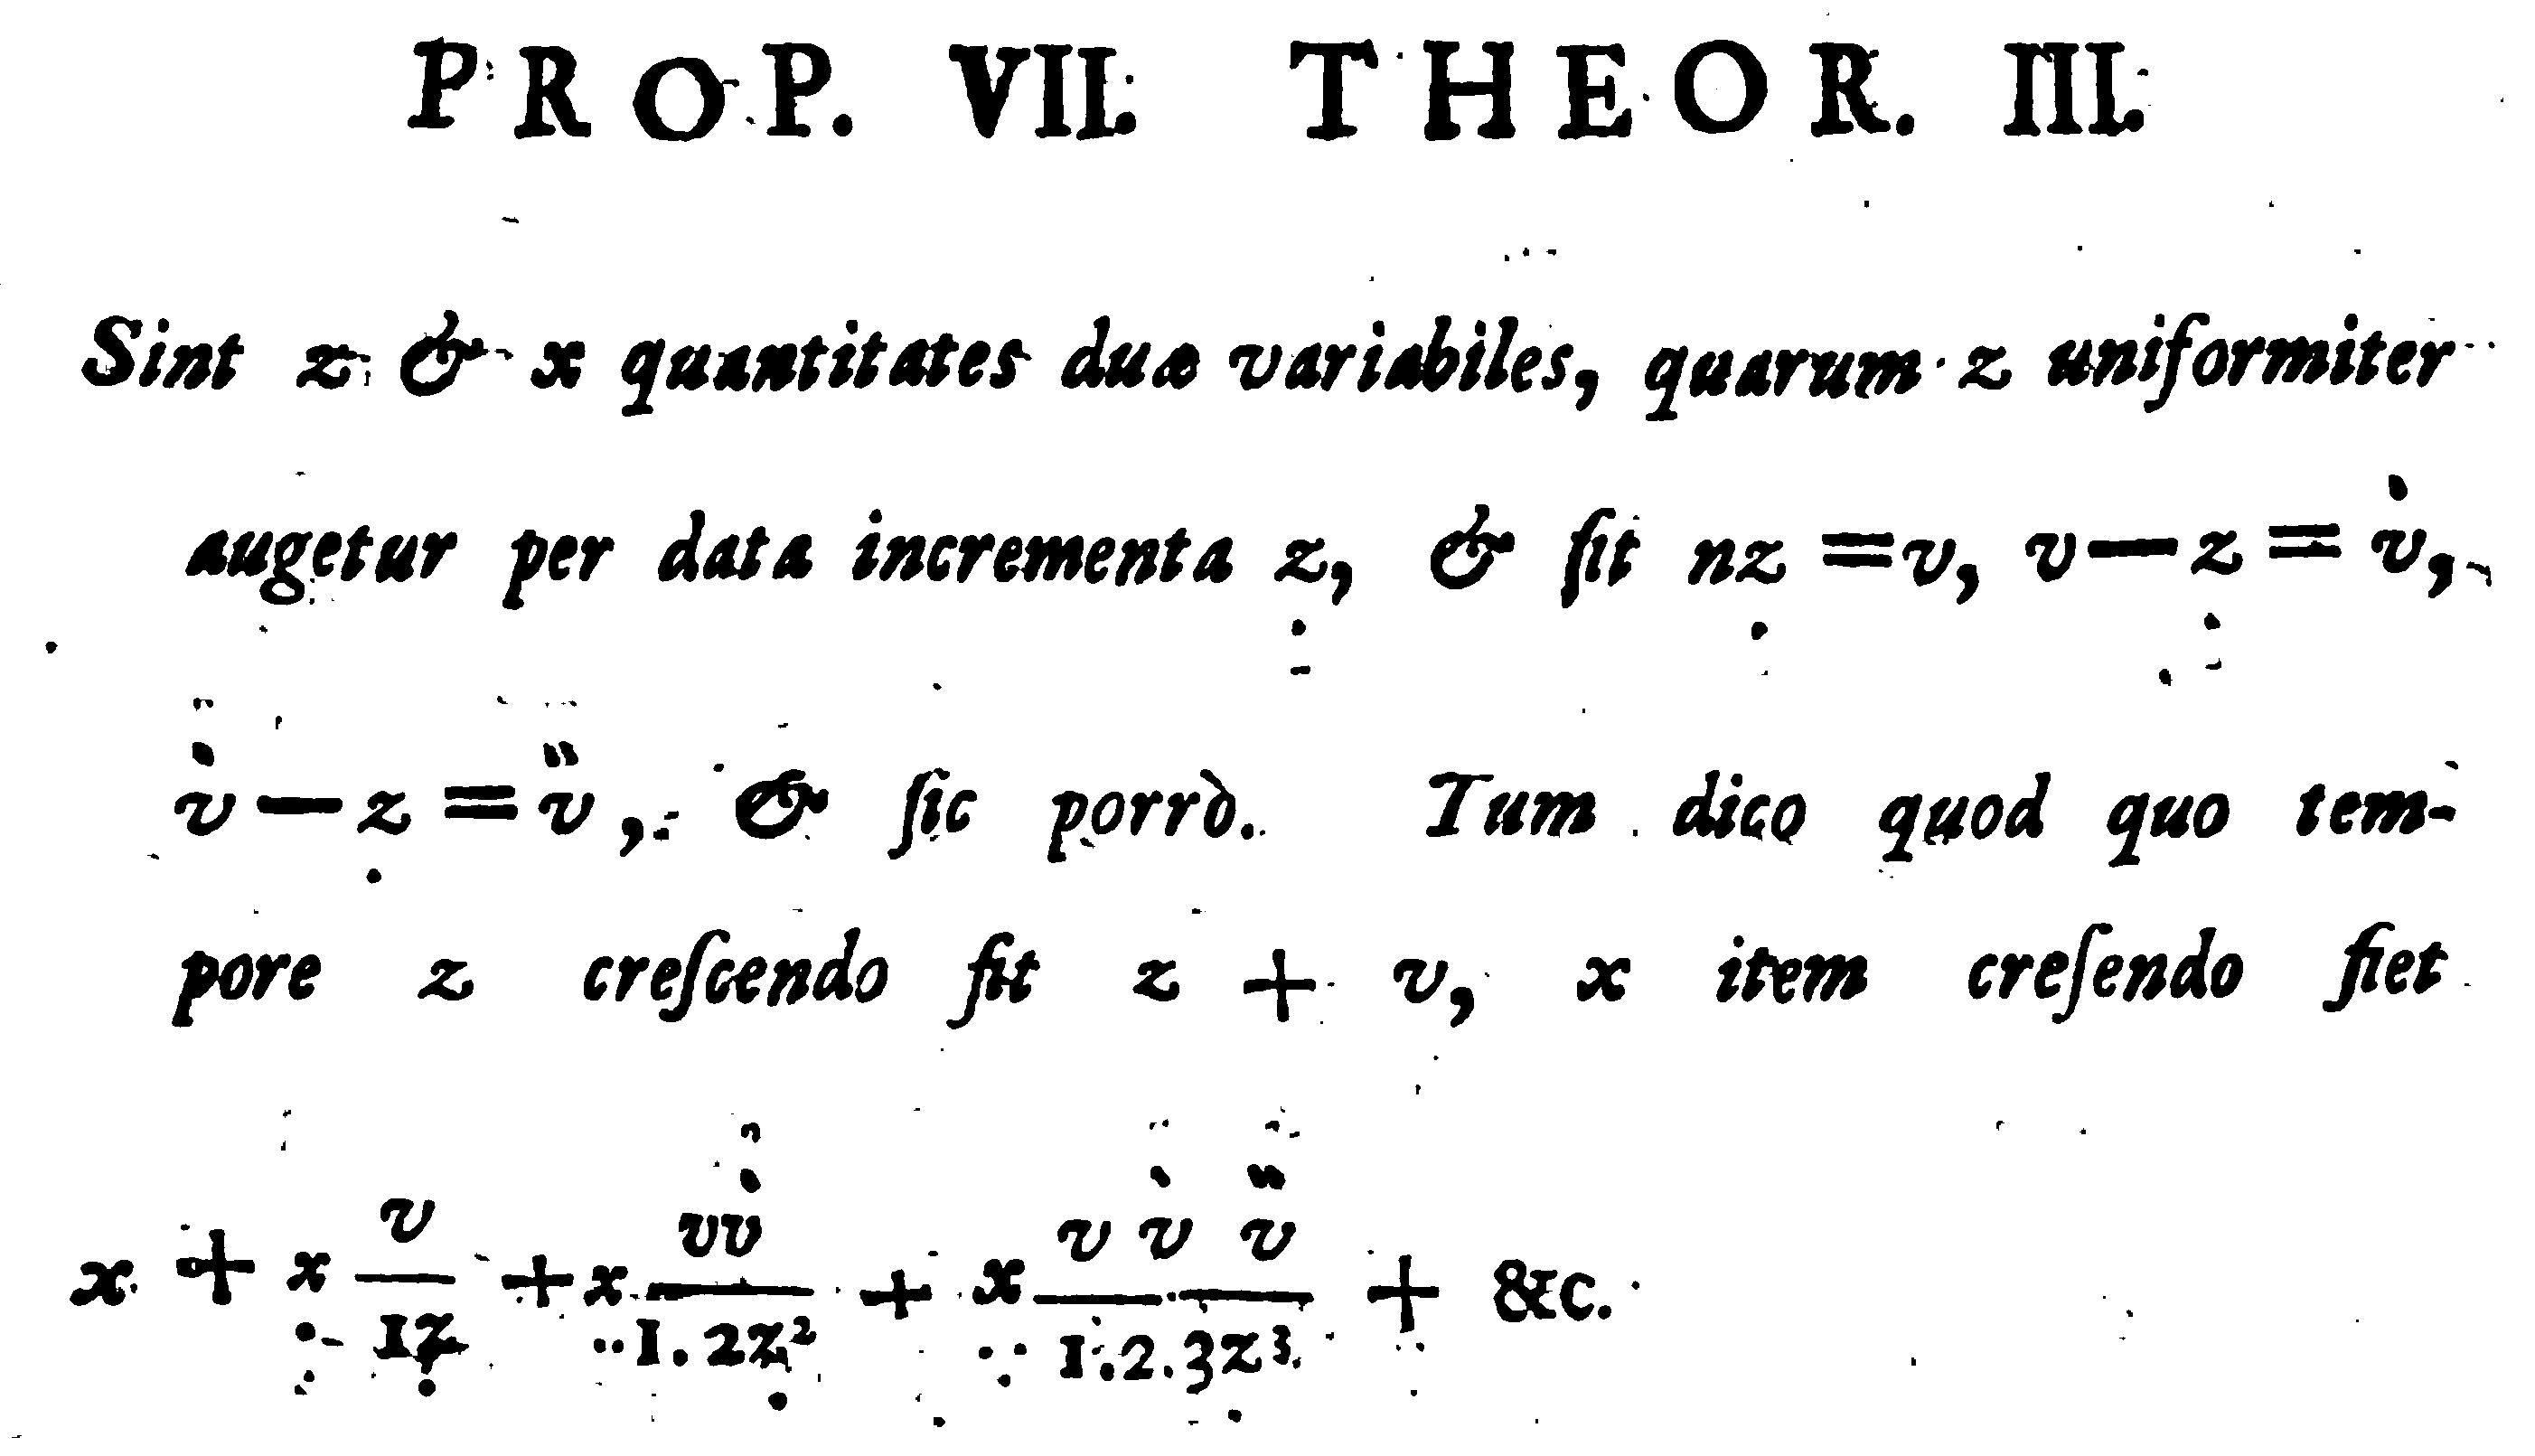
\includegraphics[scale=0.11]{figures/Taylor--MethodusPage21}
\par\end{center}

\begin{center}
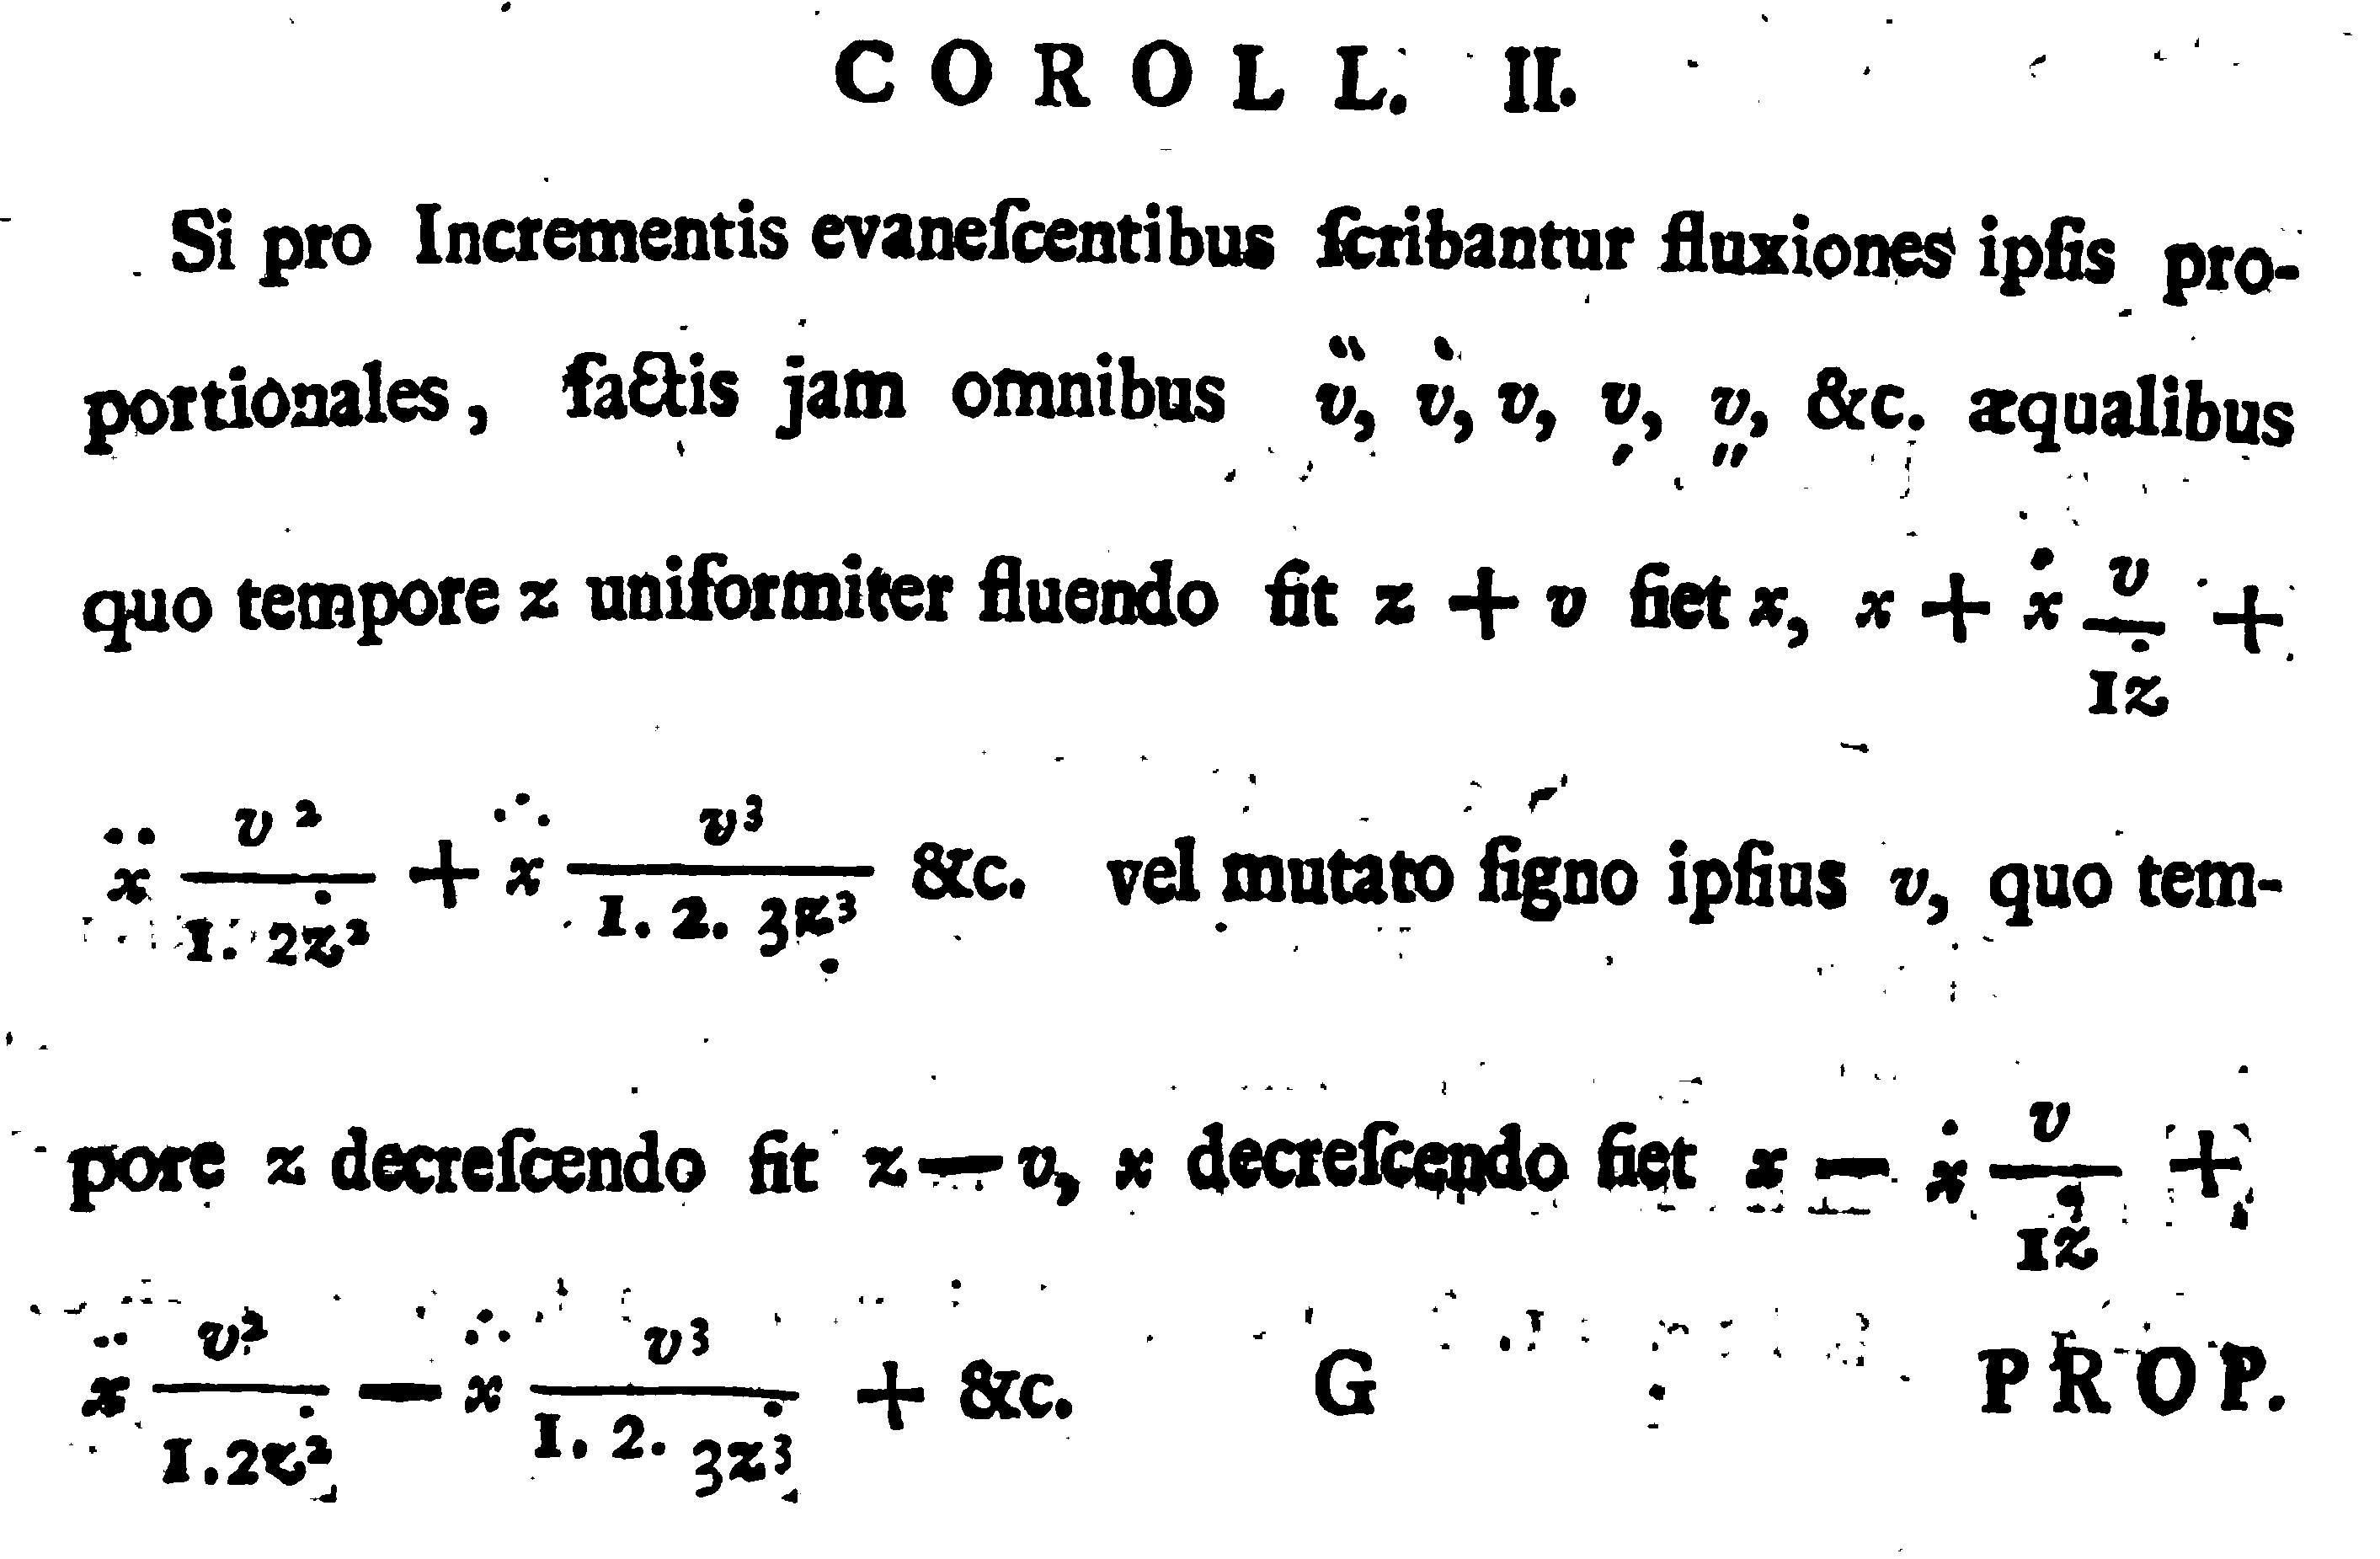
\includegraphics[scale=0.11]{figures/Taylor--MethodusPage23}
\par\end{center}

\noindent Tidak ada penyebutan suku sisa. Notasi fungsi $f(x)$ yang
lazim tidak digunakan. Teksnya ditulis dalam bahasa Latin. Dan tidak
ada daftar panjang hipotesis.

Berikut pernyataan asli teorema Taylor dalam bahasa Inggris sebagaimana
diterjemahkan oleh Ian Bruce.\textsc{ Proposisi VII. Teorema III:}
Terdapat dua besaran variabel, $z$ \& $x$, dengan $z$ bertambah
secara teratur sebesar pertambahan yang diberikan $\underset{\dot{\ }}{z}$,
dan $n\underset{\dot{\ }}{z}=v$, $v-\underset{\dot{\ }}{z}=\overset{^{\backslash}}{v}$,
$\overset{^{\backslash}}{v}-\underset{\dot{\ }}{z}=\overset{^{\backslash\backslash}}{v}$,
dan seterusnya. Selanjutnya, saya menyatakan bahwa selama waktu $z$
bertambah menjadi $z+v$, $x$ juga bertambah menjadi $x+\underset{\dot{\ }}{x}\frac{v}{1\underset{\dot{\ }}{z}}+\underset{\ddot{\ }}{x}\frac{v\overset{\backslash}{v}}{1\cdot2\underset{\dot{\ }}{z}^{2}}+\underset{\dddot{\ }}{x}\frac{v\overset{\backslash}{v}\overset{\backslash\backslash}{v}}{1\cdot2\cdot3\underset{\dot{\ }}{z}^{3}}+\mbox{\&c}$.\textsc{
Korolari II:} Jika untuk pertambahan yang melenyap, fluksion dari
besaran-besaran yang sebanding itu sendiri dituliskan, kini dengan
semua $\overset{^{\backslash\backslash}}{v},\ \overset{^{\backslash}}{v},\ v,\ \underset{^{/}}{v},\ \underset{^{//}}{v},\mbox{ \&c.}$
sama dengan waktu $z$ yang mengalir seragam hingga menjadi $z+v$,
$x$ menjadi $x+\dot{x}\frac{v}{1\dot{z}}+\ddot{x}\frac{v^{2}}{1\cdot2\dot{z}^{2}}+\dddot{x}\frac{v^{3}}{1\cdot2\cdot3\dot{z}^{3}}+\mbox{\&c }\ldots$

\end{digression}

\begin{digression}{Penafsiran teorema asli Brook Taylor} 

\noindent Sayangnya, terjemahan bahasa Inggris teorema Taylor hanya
cukup membantu bagi orang yang tidak akrab dengan matematika awal
abad ke-$18$. Pada tahun 1715, notasi fungsi masih baru akan muncul
20 tahun kemudian. Saat ini, kita akan menafsirkan deklarasi kedua
variabel itu sebagai pernyataan bahwa $x$ merupakan fungsi dari $z$.
Klaim dalam Teorema III adalah bahwa kita dapat menulis ulang $x(z+v)$
sebagai $x+\underset{\dot{\ }}{x}\frac{v}{1\underset{\dot{\ }}{z}}+\underset{\ddot{\ }}{x}\frac{v\overset{\backslash}{v}}{1\cdot2\underset{\dot{\ }}{z}^{2}}+\underset{\dddot{\ }}{x}\frac{v\overset{\backslash}{v}\overset{\backslash\backslash}{v}}{1\cdot2\cdot3\underset{\dot{\ }}{z}^{3}}+\mbox{\&c}$.
Sama seperti $x$ harus ditafsirkan sebagai fungsi dari $z$, demikian
pula $\underset{\dot{\ }}{x}$, $\underset{\ddot{\ }}{x}$, dan $\underset{\dddot{\ }}{x}$.
Lebih tepatnya, $\underset{\dot{\ }}{x}$ berarti $x(z+\underset{\dot{\ }}{z})-x(z)$,
yaitu besarnya pertambahan $x$ ketika $z$ ditambah sebesar $\underset{\dot{\ }}{z}$.
Demikian pula, $\underset{\ddot{\ }}{x}$ adalah besarnya pertambahan
$\underset{\dot{\ }}{x}$ ketika $z$ ditambah sebesar $\underset{\dot{\ }}{z}$,
sehingga $\underset{\ddot{\ }}{x}=\underset{\dot{\ }}{x}(z+\underset{\dot{\ }}{z})-\underset{\dot{\ }}{x}(z)=\left[x(z+2\underset{\dot{\ }}{z})-x(z+\underset{\dot{\ }}{z})\right]-\left[x(z+\underset{\dot{\ }}{z})-x(z)\right]=x(z+2\underset{\dot{\ }}{z})-2x(z+\underset{\dot{\ }}{z})+x(z)$.
Serupa dengan itu, $\underset{\dddot{\ }}{x}$ adalah besarnya pertambahan
$\underset{\ddot{\ }}{x}$ ketika $z$ ditambah sebesar $\underset{\dot{\ }}{z}$.
Sekarang saat yang tepat untuk berhenti membaca sejenak dan memverifikasi
bahwa $\underset{\dddot{\ }}{x}=x(z+3\underset{\dot{\ }}{z})-3x(z+2\underset{\dot{\ }}{z})+3x(z+\underset{\dot{\ }}{z})-x(z)$,
bahwa $\underset{\ddddot{\ }}{x}=x(z+4\underset{\dot{\ }}{z})-4x(z+3\underset{\dot{\ }}{z})+6x(z+2\underset{\dot{\ }}{z})-4x(z+\underset{\dot{\ }}{z})+x(z)$,
dan seterusnya. Dengan pemahaman ini serta konvensi $\underset{0}{x}$
untuk $x$, $\underset{1}{x}$ untuk $\underset{\dot{\ }}{x}$, $\underset{2}{x}$
untuk $\underset{\ddot{\ }}{x}$, $\overset{0}{v}$ untuk $v$, $\overset{1}{v}$
untuk $\overset{^{\backslash}}{v}$, $\overset{2}{v}$ untuk $\overset{^{\backslash\backslash}}{v}$,
dan seterusnya, dapat ditunjukkan melalui latihan aljabar bahwa
\begin{eqnarray*}
x(z+n\underset{\dot{\ }}{z}) & = & \sum_{j=0}^{n}\left(\begin{array}{c}
n\\
j
\end{array}\right)\underset{^{j}}{x}=\underset{^{0}}{x}+\underset{^{1}}{x}\frac{n}{1}+\underset{^{2}}{x}\frac{n(n-1)}{1\cdot2}+\underset{^{3}}{x}\frac{n(n-1)(n-2)}{1\cdot2\cdot3}+\cdots+\underset{^{n}}{x}\frac{n(n-1)\cdots1}{1\cdot2\cdot3\cdots n}\\
 & = & \underset{^{0}}{x}+\underset{^{1}}{x}\frac{n\underset{\dot{\ }}{z}}{1\underset{\dot{\ }}{z}}+\underset{^{2}}{x}\frac{n\underset{\dot{\ }}{z}(n-1)\underset{\dot{\ }}{z}}{1\cdot2\underset{\dot{\ }}{z}^{2}}+\underset{^{3}}{x}\frac{n\underset{\dot{\ }}{z}(n-1)\underset{\dot{\ }}{z}(n-2)\underset{\dot{\ }}{z}}{1\cdot2\cdot3\underset{\dot{\ }}{z}^{3}}+\cdots+\underset{^{n}}{x}\frac{n\underset{\dot{\ }}{z}(n-1)\underset{\dot{\ }}{z}\cdots1\underset{\dot{\ }}{z}}{1\cdot2\cdot3\cdots n\underset{\dot{\ }}{z}^{n}}\\
 & = & \underset{^{0}}{x}+\underset{^{1}}{x}\frac{v}{1\underset{\dot{\ }}{z}}+\underset{^{2}}{x}\frac{v\overset{1}{v}}{1\cdot2\underset{\dot{\ }}{z}^{2}}+\underset{^{3}}{x}\frac{v\overset{2}{v}\overset{3}{v}}{1\cdot2\cdot3\underset{\dot{\ }}{z}^{3}}+\cdots+\underset{^{n}}{x}\frac{v\overset{2}{v}\overset{3}{v}\cdots\overset{n}{v}}{1\cdot2\cdot3\cdots n\underset{\dot{\ }}{z}^{n}}.
\end{eqnarray*}
Perhitungan ini pada dasarnya merupakan pembuktian Taylor untuk Teorema
III. 

Korolari II (yang akan kita anggap sebagai teorema) tidak dibuktikan
oleh Taylor selain melalui penerapan yang ``jelas'' dari teori fluksion
Newton. Dalam bahasa sekarang, Korolari II diperoleh dengan mengambil
limit ketika $n\to\infty$ pada ekspresi dari Teorema III. Latihan
menarik lainnya adalah memverifikasi bahwa $\lim_{n\to\infty}\frac{\underset{k}{x}}{\underset{\dot{\ }}{z}^{k}}=x^{(k)}(z)$,
yaitu turunan berorde $k$ dari $x$. Dan satu latihan terakhir untuk
melihat bahwa $\lim_{n\to\infty}\overset{k}{v}=v$. Sebagaimana Taylor
menganggap hasil-hasil ini begitu saja, demikian pula kita. Dengan
menerapkannya pada Teorema III, kita memperoleh $x(z+v)=x(z)+x'(z)\frac{v}{1!}+x''(z)\frac{v^{2}}{2!}+x'''(z)\frac{v^{3}}{3!}+\cdots$.
Dalam notasi Taylor, $\frac{\dot{x}}{\dot{z}}$ adalah turunan pertama
dari $x$, $\frac{\ddot{x}}{\dot{z}^{2}}$ adalah turunan kedua dari
$x$, dan seterusnya. Jadi, kita memang memperoleh $x+\dot{x}\frac{v}{1\dot{z}}+\ddot{x}\frac{v^{2}}{1\cdot2\dot{z}^{2}}+\dddot{x}\frac{v^{3}}{1\cdot2\cdot3\dot{z}^{3}}+\mbox{\&c}$
sebagaimana diklaim.

Menarik bahwa Teorema III berlaku untuk fungsi $x$ apa pun yang didefinisikan
pada interval $[x,x+v]$. Tidak menjadi masalah apakah $x$ terdiferensialkan,
atau bahkan kontinu. Teorema ini merupakan pernyataan tentang beda
hingga. Justru korolarinya memerlukan jauh lebih banyak asumsi karena
di sanalah kita beralih ke limit. \end{digression} 

\subsection{Octave}

Dua hal yang akan berulang kali berguna ketika menggunakan Octave
adalah fungsi anonim \index{Octave!fungsi anonim} dan berkas \texttt{.m}\index{Octave!berkas .m@berkas \texttt{.m}}.
Membuat fungsi anonim merupakan cara sederhana untuk membuat fungsi
``khusus'' dalam Octave. Membuat berkas \texttt{.m} merupakan cara
yang teratur untuk menjalankan sejumlah perintah dan menyimpan pekerjaan
Anda untuk digunakan kemudian. 

Pada bagian sebelumnya kita melihat banyak fungsi bawaan seperti \texttt{sin(x)},
\texttt{log(x)}, dan \texttt{abs(x)}. Fungsi-fungsi ini memiliki makna
yang telah ditentukan dalam Octave. Namun, bagaimana jika Anda ingin
mendefinisikan $f(x)=3x^{2}$? Tidak ada fungsi bawaan ``3 $x$ kuadrat''.
Di sinilah fungsi anonim berguna. Sintaks fungsi anonim adalah

\begin{center}
\texttt{nama = @(variabel) definisi fungsi}
\par\end{center}

\noindent di mana \texttt{nama} adalah nama fungsi,\texttt{ variabel}
adalah daftar variabel yang digunakan dalam fungsi dan dipisahkan
dengan koma, sedangkan \texttt{definisi fungsi} adalah rumusnya. Untuk
$f(x)=3x^{2}$, kode Octave-nya adalah \texttt{f=@(x) 3{*}x\textasciicircum 2}.
Selanjutnya Anda dapat menggunakan \texttt{f} dengan cara yang sama
seperti menggunakan \texttt{sin}, \texttt{log} atau \texttt{abs}.
Ketik nama fungsi, tanda kurung buka, argumen, lalu tanda kurung tutup.
Jadi, setelah mendefinisikan \texttt{f} dengan pernyataan \texttt{f=@(x)
3{*}x\textasciicircum 2}, \texttt{f(7)} akan menghasilkan 147: \begin{verbatim}
octave:1> f=@(x) 3*x^2;
octave:2> f(7)
ans =  147 
\end{verbatim}

Sekarang kita dapat menyelesaikan Percobaan 1 pada bagian \ref{sec:Accuracy}
dengan cara keempat. Alih-alih melakukan perhitungan pada baris perintah,
kita dapat membuat berkas teks yang memuat perintah-perintah tersebut.
Setelah disimpan sebagai berkas \texttt{.m}, Octave akan mengenalinya
sebagai daftar instruksi. Jika Anda terbiasa dengan pemrograman, cara
bekerja dengan Octave ini akan terasa sangat alami. Menulis berkas
\texttt{.m} setara dengan menulis sebuah program. Setelah ditulis,
berkas tersebut perlu diproses. Pada baris perintah Octave, berkas
\texttt{.m} dijalankan dengan mengetikkan nama berkas tanpa akhiran
\texttt{.m}. Hanya itu, sehingga prosesnya tidak persis seperti menulis
sebuah program. Tidak ada proses kompilasi. Dalam hal ini, prosesnya
lebih menyerupai pembuatan skrip. 

Untuk memulai, gunakan editor teks apa pun yang Anda sukai untuk membuat
daftar perintah. Perhatikan baik-baik: Microsoft Word, LibreOffice,
dan pengolah kata lainnya bukanlah editor teks. Program-program tersebut
adalah pengolah kata. Pengolah kata memiliki fitur pemformatan huruf,
pengaturan halaman, dan sebagainya. Sekarang bayangkan laporan terakhir
atau surat Anda kepada Ibu, lalu hapus semua pemformatannya kecuali
pemisah antarparagraf. Itulah berkas teks. Tidak ada cetak tebal,
pemusatan, gambar, huruf khusus, margin, ataupun halaman. Hanya kata-kata
yang diketik. Segala hiasan yang disediakan pengolah kata tidak diperlukan.
Octave hanya memerlukan daftar perintah. Pemformatan yang diperlukan
hanyalah ganti baris dan tab. Jika Anda belum memiliki editor teks
favorit---dan mungkin sekalipun sudah---gunakanlah editor yang disertakan
bersama Octave. Dengan program tersebut, Anda tidak akan mengalami
masalah. Jika Anda menggunakan Octave Online atau CoCalc, platform
daring itu menyediakan editor; gunakanlah editor tersebut. 

Dengan editor teks pilihan Anda, buatlah dokumen teks \texttt{experiment1.m}
persis seperti yang ditampilkan berikut ini: \begin{verbatim}
format('long')
p1 = 10*pi-31
p2 = 100*p1-41
p3 = 100*p2-59
p4 = 100*p3-26
p5 = 100*p4-53
p6 = 100*p5-58
p7 = 100*p6-97 
\end{verbatim} Kemudian, pada baris perintah Octave, ketik \texttt{experiment1}
untuk memperoleh hasilnya: \begin{verbatim}
octave:1> experiment1
p1 =  0.415926535897931
p2 =  0.592653589793116
p3 =  0.265358979311600
p4 =  0.535897931159980
p5 =  0.589793115997963
p6 =  0.979311599796347
p7 =  0.931159979634685
\end{verbatim} Cara menulis perintah Octave ini memiliki dua keunggulan yang jelas.
Pertama, jika Anda membuat kesalahan, memperbaikinya sangat mudah.
Cukup sunting berkas teks tersebut dan simpan perubahannya. Kedua,
Anda memiliki catatan pekerjaan Anda. Anda dapat membagikan, mencetak,
atau sekadar menyimpannya untuk digunakan kemudian. Hanya ada satu
kekurangan nyata. Cara ini lebih rumit daripada sekadar menjalankan
beberapa perintah pada baris perintah. Karena itu, untuk perhitungan
sederhana, cara ini lebih merepotkan daripada yang diperlukan.

Perhatikan bahwa berkas \texttt{.m} harus disimpan dalam direktori
yang sama dengan tempat Octave dijalankan. Jika Anda menggunakan lingkungan
pengembangan terintegrasi (IDE), perincian semacam ini akan ditangani
untuk Anda. Namun, jika Anda menggunakan baris perintah dan editor
teks, pastikan berkas \texttt{.m} disimpan di lokasi yang benar.

\noindent\startexercises

\subsection{Latihan}
\begin{enumerate}
\item Tentukan $T_{3}(x)$ dan $R_{3}(x)$ untuk fungsi yang dikembangkan
di sekitar $x_{0}$.

\begin{enumerate}
\item \label{exc:taylor1}$f(x)=\sin(x)$; $x_{0}=0$. \hasasolution 
\item $f(x)=\sin(x)$; $x_{0}=\pi/2$.
\item \label{exc:taylor2}$f(x)=\sin(x)$; $x_{0}=\pi$. \hasasolution 
\item $f(x)=e^{x}$; $x_{0}=0$.
\item $f(x)=e^{x}$; $x_{0}=\ln2$.
\item \label{exc:taylor3}$f(x)=x\sin(x)$; $x_{0}=0$. \hasananswer 
\item $f(x)=\cos^{2}(x)$; $x_{0}=0$.
\end{enumerate}
\item Misalkan $f(x)=4x^{3}-2x^{2}+8x-9$.

\begin{enumerate}
\item Tentukan $T_{3}(x)$ dan $R_{3}(x)$ untuk pengembangan di sekitar
$x_{0}=0$.
\item Tentukan $T_{3}(x)$ dan $R_{3}(x)$ untuk pengembangan di sekitar
$x_{0}=2$.
\item Rumuskan suatu konjektur berdasarkan jawaban Anda untuk bagian (a)
dan (b). Dapatkah Anda membuktikannya?
\end{enumerate}
\item Tentukan polinomial Maclaurin berindeks $36$ untuk $f(x)=e^{x}$.
\item Misalkan $f(x)$ adalah fungsi yang memiliki turunan keempat pada
seluruh garis bilangan real, $(-\infty,\infty)$, dan memenuhi $f(2)=3$,
$f'(2)=-1$, $f''(2)=2$, serta $f'''(2)=-1$.

\begin{enumerate}
\item Tuliskan polinomial Taylor derajat ketiga untuk $f(x)$ yang dikembangkan
di sekitar $x_{0}=2$.
\item Gunakan polinomial Taylor tersebut untuk menghampiri $f(4)$.
\item Tentukan suatu batas atas bagi galat absolut hampiran tersebut dengan
memanfaatkan fakta bahwa
\[
-3\leq f^{(4)}(\xi)\leq5
\]
untuk setiap $\xi\in[2,4]$.
\end{enumerate}
\item Hitung polinomial Taylor berindeks $3$ untuk $f(x)=x^{5}-2x^{4}+x^{3}-9x^{2}+x-1$
yang dikembangkan di sekitar $x_{0}=1$.
\item Tentukan polinomial Taylor derajat kedua untuk $f(x)=\csc x$ yang
dikembangkan di sekitar ${\displaystyle x_{0}=\frac{\pi}{4}}$. Berikut
beberapa fakta yang mungkin berguna:
\begin{gather*}
f'(x)=-\csc(x)\cot(x)\quad\csc(x)=\frac{1}{\sin(x)}\\
f''(x)=\csc(x)(1+2\cot^{2}(x))\quad\cot(x)=\frac{\cos(x)}{\sin(x)}
\end{gather*}
\item Sinus hiperbolik, $\sinh(x)$, dan kosinus hiperbolik, $\cosh(x)$,
saling merupakan turunan. Artinya, 
\[
\begin{gathered}\frac{\textrm{d}}{\textrm{d}x}(\sinh(x))=\cosh(x)\\
\textrm{dan}\\
\frac{\textrm{d}}{\textrm{d}x}(\cosh(x))=\sinh(x).
\end{gathered}
\]
Tentukan suku sisa, $R_{43}$, yang terkait dengan polinomial Maclaurin
berindeks $43$ untuk $f(x)=\cosh(x)$. 
\item \octave\ \label{exc:taylor8}Gunakan fungsi anonim untuk menghitung
nilai polinomial Taylor $T_{4}(x)=1-\frac{1}{2}x^{2}+\frac{1}{24}x^{4}$
pada nilai $x$ yang diberikan. \hasasolution 

\begin{enumerate}
\item 0
\item $\frac{1}{2}$
\item 1
\item $\pi$
\end{enumerate}
\item \octave\ \label{exc:taylor10}Gunakan fungsi anonim untuk menghitung
nilai polinomial Taylor $T_{3}(x)=1+x+\frac{1}{2}x^{2}+\frac{1}{6}x^{3}$
pada nilai $x$ yang diberikan.

\begin{enumerate}
\item 0
\item $\frac{3}{2}$
\item $2$
\item \label{exc:taylor9}$e$ \hasananswer 
\end{enumerate}
\item \octave\ \label{exc:taylor11}Tulis dan jalankan sebuah berkas \texttt{.m}
yang menghitung semua jawaban untuk latihan \ref{exc:taylor8}. \hasasolution 
\item \octave\ Tulis dan jalankan sebuah berkas \texttt{.m} yang menghitung
semua jawaban untuk latihan \ref{exc:taylor10}.
\item Tentukan $\xi(x)$ yang keberadaannya dijamin oleh teorema Taylor
dalam setiap situasi berikut.

\begin{enumerate}
\item \label{exc:taylor7}$f(x)=\cos(x)$, $x_{0}=0$, $n=3$, $x=\pi$. \hasananswer 
\item $f(x)=e^{x}$, $x_{0}=0$, $n=3$, $x=\ln4$.
\item $f(x)=\ln(x)$, $x_{0}=1$, $n=4$, $x=2$.
\end{enumerate}
\item Misalkan $f(x)=x^{3}$.

\begin{enumerate}
\item Tentukan polinomial Taylor derajat kedua, $P_{2}(x)$, yang dikembangkan
di sekitar $x_{0}=0$.
\item Tentukan suku sisa, $R_{2}(0.5)$, serta galat sebenarnya yang timbul
ketika $P_{2}(0.5)$ digunakan untuk menghampiri $f(0.5)$.
\item Ulangi bagian (a) dengan menggunakan $x_{0}=1$.
\item Ulangi bagian (b) dengan menggunakan polinomial dari bagian (c).
\end{enumerate}
\item Tentukan polinomial Taylor derajat kedua, $P_{2}(x)$, untuk $f(x)=e^{x}\cos x$
yang dikembangkan di sekitar $x_{0}=0$.

\begin{enumerate}
\item Gunakan $P_{2}(0.5)$ untuk menghampiri $f(0.5)$. Tentukan batas
atas bagi galat $|f(0.5)-P_{2}(0.5)|$ dengan menggunakan suku sisa,
lalu bandingkan batas tersebut dengan galat sebenarnya.
\item Tentukan suatu batas bagi galat $|f(x)-P_{2}(x)|$ yang berlaku untuk
seluruh interval $[0,1]$.
\item Hampiri $\int_{0}^{1}f(x)\,dx$ dengan menghitung $\int_{0}^{1}P_{2}(x)\,dx$
sebagai gantinya.
\item Tentukan batas atas bagi galat pada bagian (c) dengan menggunakan
$\int_{0}^{1}|R_{2}(x)|\,dx$ dan bandingkan batas tersebut dengan
galat sebenarnya.
\end{enumerate}
\item Misalkan $f(x)=e^{x}$.

\begin{enumerate}
\item Tentukan polinomial Maclaurin berindeks $n$ $P_{n}(x)$ untuk $f(x)$.
\item Tentukan batas galat ketika $P_{4}(2)$ digunakan untuk menghampiri
$f(2)$.
\item Berapa banyak suku polinomial Maclaurin yang perlu digunakan untuk
menghampiri $f(2)$ dengan galat tidak lebih dari $10^{-10}$? Dengan
kata lain, untuk nilai $n$ berapakah $P_{n}(2)$ memiliki batas galat
yang kurang dari atau sama dengan $10^{-10}$?
\end{enumerate}
\item Tentukan polinomial Taylor derajat keempat untuk $\ln x$ yang dikembangkan
di sekitar $x_{0}=1$. 
\item Apa suku berindeks $50$ dari $T_{100}(e^{x})$ yang dikembangkan
di sekitar $x_{0}=6$?
\item \label{arctan}Deret Maclaurin untuk fungsi arkustangen konvergen
pada $-1<x\leq1$ dan diberikan oleh
\[
\arctan x=\lim_{n\to\infty}P_{n}(x)=\lim_{n\to\infty}\sum_{i=1}^{n}(-1)^{i-1}\frac{x^{2i-1}}{2i-1}.
\]
Gunakan fakta bahwa $\tan(\pi/4)=1$ untuk menentukan banyaknya suku,
$n$, dalam deret yang harus dijumlahkan untuk memastikan bahwa $|4P_{n}(1)-\pi|<10^{-3}$.
\item Latihan \ref{arctan} menguraikan cara yang kurang efisien untuk memperoleh
hampiran bagi $\pi$. Metode tersebut dapat diperbaiki secara berarti
dengan mengamati bahwa $\pi/4=\arctan\frac{1}{2}+\arctan\frac{1}{3}$
serta menghitung deret arkustangen pada $\frac{1}{2}$ dan pada $\frac{1}{3}$.
Tentukan banyaknya suku yang harus dijumlahkan agar diperoleh hampiran
bagi $\pi$ dengan galat tidak lebih dari $10^{-3}$.
\item Untuk $f(x)=\tan^{-1}(x)$, 
\[
f^{(n)}(0)=\begin{cases}
0 & \textrm{jika }n\textrm{ genap}\\
(-1)^{(n-1)/2}(n-1)! & \textrm{jika }n\textrm{ ganjil}.
\end{cases}
\]
tentukan polinomial Maclaurin berindeks $n$ $P_{n}(x)$ untuk $f$.
\item Berapa banyak suku deret Maclaurin untuk $\sin x$ yang diperlukan
untuk menjamin hampiran dengan galat tidak lebih dari $10^{-2}$ bagi
setiap nilai $x$ antara 0 dan $2\pi$?
\item Misalkan Anda menghampiri $f(x)=e^{x}$ menggunakan polinomial Maclaurin
derajat kesepuluh. Tentukan interval terbesar yang menjamin hampiran
tersebut memiliki galat tidak lebih dari $10^{-3}$.
\item Tentukan batas galat dalam menghampiri $e^{10}$ dengan menggunakan
polinomial Taylor derajat kedua puluh lima dari $g(x)=e^{x}$ yang
dikembangkan di sekitar $x_{0}=0$.
\item Tentukan batas galat hampiran 
\[
e^{2}\approx1+2+\frac{1}{2}(2)^{2}+\frac{1}{6}(2)^{3}+\frac{1}{24}(2)^{4}+\frac{1}{120}(2)^{5}
\]
menurut teorema Taylor. Bandingkan batas ini dengan galat sebenarnya.
\item Misalkan $f^{(8)}(x)=e^{x}\cos x$ untuk suatu fungsi $f$. Tentukan
batas galat dalam menghampiri $f(x)$ pada interval $[0,\pi/2]$ dengan
menggunakan $T_{7}(x)$ yang dikembangkan di sekitar $x_{0}=0$.
\item \label{exc:taylor4}Misalkan $f(x)=\frac{1}{x}$, dan $x_{0}=5$. \hasasolution 

\begin{enumerate}
\item Tentukan $T_{2}(x)$.
\item Tentukan $R_{2}(x)$.
\item Gunakan $T_{2}(x)$ untuk menghampiri $f(1)$ dan $f(9)$.
\item Tentukan batas atas teoretis bagi galat absolut setiap hampiran pada
bagian (c).
\item Tentukan batas bawah teoretis bagi galat absolut setiap hampiran pada
bagian (c).
\item Tentukan galat absolut sebenarnya untuk setiap hampiran pada bagian
(c). Verifikasi bahwa galat-galat tersebut memang berada di antara
batas-batas teoretis.
\item Buat sketsa grafik $f(x)$ dan $T_{2}(x)$ pada sistem sumbu yang
sama untuk $x\in[1,9]$.
\end{enumerate}
\item Misalkan $f(x)=\ln(1+x)$ dan $x_{0}=0$.

\begin{enumerate}
\item Tentukan $T_{3}(x)$.
\item Tentukan $R_{3}(x)$.
\item Gunakan $T_{3}(x)$ untuk menghampiri $f(1)$ dan $f(26)$.
\item Tentukan batas atas teoretis bagi galat absolut setiap hampiran pada
bagian (c).
\item Tentukan batas bawah teoretis bagi galat absolut setiap hampiran pada
bagian (c).
\item Tentukan galat absolut sebenarnya untuk setiap hampiran pada bagian
(c). Verifikasi bahwa galat-galat tersebut memang berada di antara
batas-batas teoretis.
\item Buat sketsa grafik $f(x)$ dan $T_{3}(x)$ pada sistem sumbu yang
sama untuk $x\in[1,26]$.
\end{enumerate}
\item Misalkan $f(x)$ memenuhi $-3\leq f^{(10)}(x)\leq7$ untuk setiap
$x\in[0,10]$. Tentukan batas bawah dan batas atas bagi galat absolut
ketika $T_{9}(x)$ yang dikembangkan di sekitar $x_{0}=3$ digunakan
untuk menghampiri

\begin{enumerate}
\item $f(0)$.
\item $f(10)$.
\end{enumerate}
\item Misalkan Anda ingin menghampiri nilai $-e^{4}\sin4$ dengan menggunakan
polinomial Maclaurin terpisah (polinomial Taylor yang dikembangkan
di sekitar $x_{0}=0$) untuk fungsi sinus dan eksponensial, alih-alih
menggunakan satu polinomial Maclaurin untuk fungsi $f(x)=-e^{x}\sin x$.
Berapa banyak suku dari masing-masing polinomial yang diperlukan untuk
memperoleh galat tidak lebih dari $10^{-20}$? Abaikan galat pembulatan.
\item Tentukan batas atas teoretis, sebagai fungsi dari $x$, bagi galat
absolut ketika $T_{4}(x)$ digunakan untuk menghampiri $f(x)$.

\begin{enumerate}
\item $e^{x}\sin x$; $x_{0}=0$.
\item \label{exc:taylor5}$e^{-x^{2}}$; $x_{0}=0$. \hasasolution 
\item $\frac{10}{x}+\sin(10x)$; $x_{0}=\pi$.
\end{enumerate}
\item Deret Maclaurin untuk $f(x)=e^{-x}$ adalah
\[
\sum_{i=0}^{\infty}\frac{(-1)^{i}}{i!}x^{i}=1-x+\frac{1}{2}x^{2}-\frac{1}{6}x^{3}+\ldots
\]
 Tentukan batas galat dalam menghampiri $1/e$ dengan $1-1+1/2-1/6+1/24$.
\item Deret Taylor untuk $f(x)=e^{x}$ adalah ${\displaystyle T(x)=1+x+\frac{1}{2!}x^{2}+\frac{1}{3!}x^{3}+\frac{1}{4!}x^{4}+\frac{1}{5!}x^{5}+\cdots}$.
Deret ini konvergen ke $f(x)$ untuk semua nilai $x$. Khususnya,
untuk $x=1$, hal ini berarti bahwa
\[
f(1)=T(1)=1+1+\frac{1}{2!}(1)^{2}+\frac{1}{3!}(1)^{3}+\frac{1}{4!}(1)^{4}+\cdots
\]
Dengan menyederhanakan persamaan ini, kita memperoleh
\[
e=1+1+\frac{1}{2}+\frac{1}{6}+\frac{1}{24}+\frac{1}{120}+\cdots
\]
Gunakan deret Taylor untuk menentukan deret tak hingga yang jumlahnya
sama dengan 

\begin{enumerate}
\item $\ln(2)$
\item $2/3$
\item $\pi/4$
\item $\sqrt{2}$
\end{enumerate}
\end{enumerate}
\finishexercises
